\documentclass[a4paper]{article}
\usepackage[utf8]{inputenc}
\usepackage{amsmath}
\usepackage{amssymb}
\usepackage{mathtools}
\usepackage{amsfonts}
\usepackage{lastpage}
\usepackage{tikz}
\usetikzlibrary{patterns}
\usepackage{pdfpages}
\usepackage{gauss}
\usepackage{fancyvrb}
\usepackage[table]{colortbl}
\usepackage{fancyhdr}
\usepackage{graphicx}
\usepackage[margin=2.5 cm]{geometry}
\pagestyle{fancy}
\def\checkmark{\tikz\fill[scale=0.4](0,.35) -- (.25,0) -- (1,.7) -- (.25,.15) -- cycle;} 
\newcommand*\circled[1]{\tikz[baseline=(char.base)]{
            \node[shape=circle,draw,inner sep=2pt] (char) {#1};}}
\newcommand*\squared[1]{%
  \tikz[baseline=(R.base)]\node[draw,rectangle,inner sep=0.5pt](R) {#1};\!}
\cfoot{Page \thepage\ of \pageref{LastPage}}
\DeclareGraphicsExtensions{.pdf,.png,.jpg}
\author{Nikolaj Dybdahl Rathcke (rfq695)}
\title{Third Home Assignment \\ Data Analysis}
\lhead{Nikolaj Dybdahl Rathcke (rfq695)}
\chead{Data Analysis}
\rhead{Assignment 3}

\begin{document}
\maketitle
\section*{Question 1}
\subsection*{(1)}
The example diatom can be seen below, generated with the code in \texttt{q1\_1}.
\begin{center}
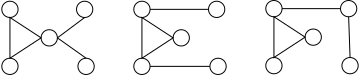
\includegraphics[scale=0.3]{fig1}
\end{center}
We can calculate the mean of the diatoms witih the code from \texttt{q1\_1b} which will provide the following figure
\begin{center}
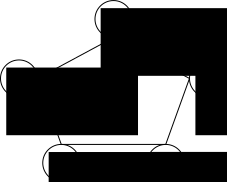
\includegraphics[scale=0.3]{fig2}
\end{center}
The sample covariance matrix can be calculated with the centered data matrix using equation (9.1). It is computed with code from \texttt{q1\_1c}.

\subsection*{(2)}
The implementation of PCA is located in \texttt{svd\_pca} and is based on the algorithm on page 12, chapter 9. It takes an $X$ matrix and an int $k$ and returns the PCA feature matrix $Z$ and the reconstructed data $\hat{X}$ .

\subsection*{(3)}
The PCA feature matrix is actually calculated in \texttt{svd\_pca} using the formula $Z = XV_k$ while the reconstructed data is calculated as $\hat{X} = XV_kV^t_k$.\\
The code in \texttt{q1\_3} calculates the reconstructed data and plots the first $3$ rows along with the first $3$ rows from the original diatoms set. This provides the following figure
\begin{center}
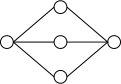
\includegraphics[scale=0.4]{fig3}
\end{center}
Where blue lines indicate the rows from the original diatoms set while the red lines indicate the rows from the reconstructed data.

\subsection*{(4)}
We use the sample covariance matrix we found in (1) (code is duplicated into file \texttt{q1\_4}). Using the eigenvalue of the matrix, we can make a spectrum plot.\\
We want to find how many principal components we need to capture 95\% of the variance of the diatoms. An initial plot with $I=20$ shows that we need around $3$ principal components. The following plot is with $I=5$
\begin{center}
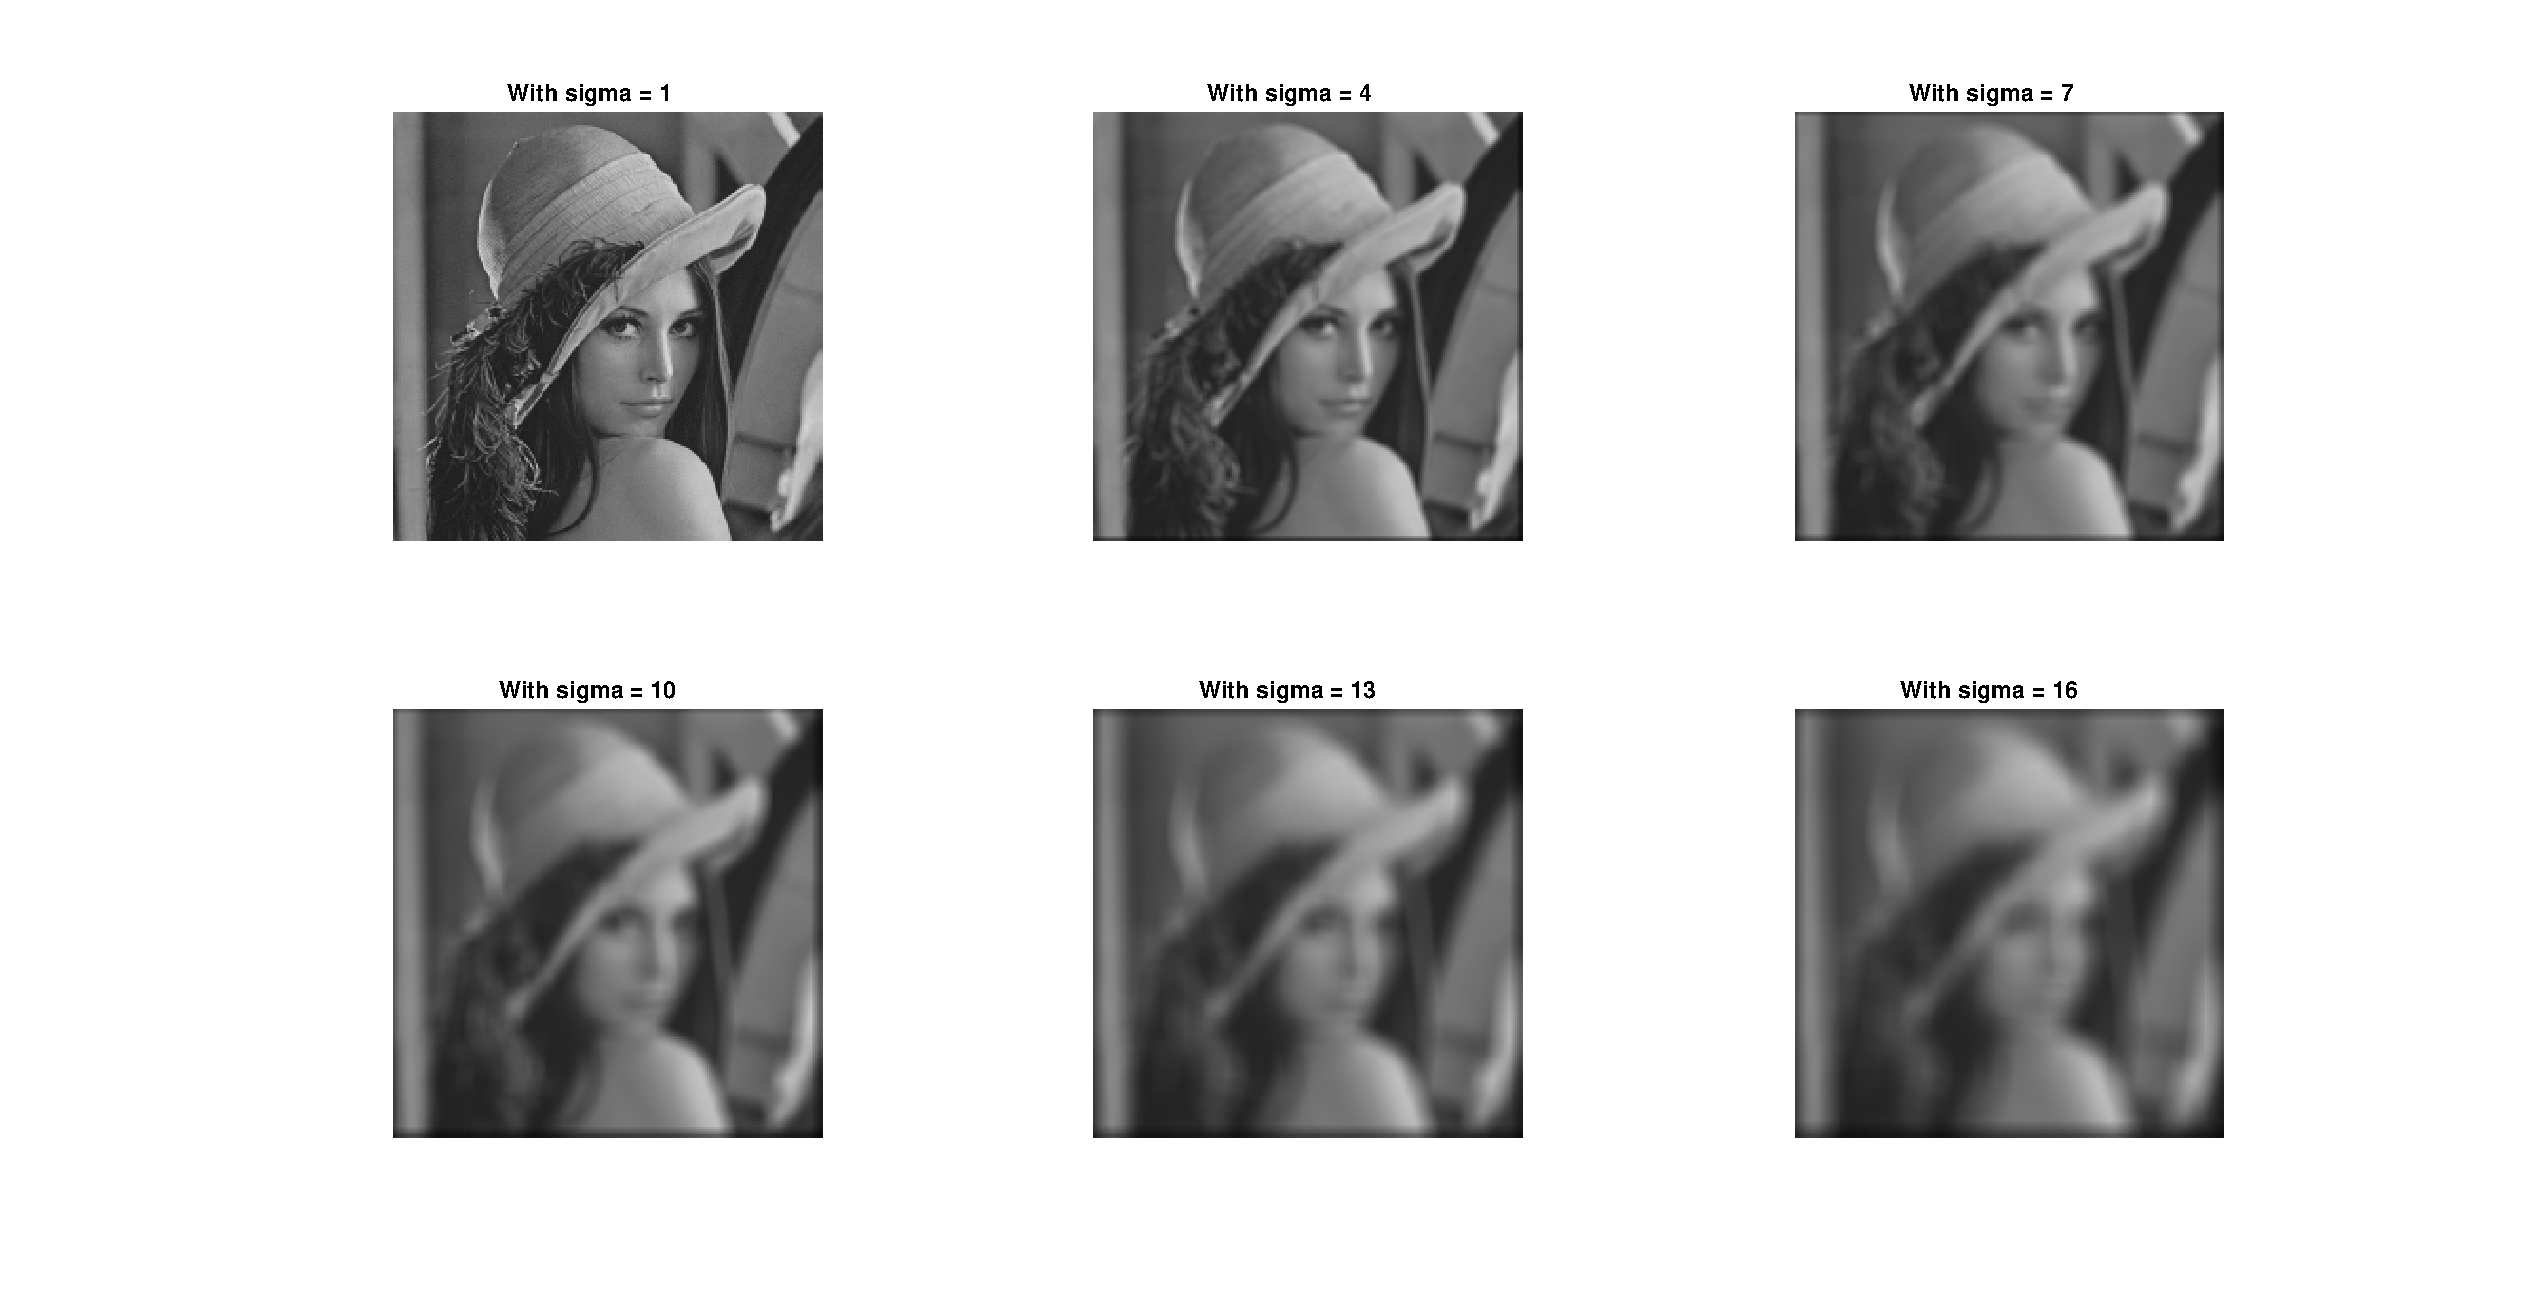
\includegraphics[scale=0.35]{fig4}
\end{center}
Where we can see we actually need $3$ principal components. This is verified by finding $spec(3)$ in \texttt{q1\_4} which returns $0.9521$.

\subsection*{(5)}
The code that visualizes the variance in the first three principal components can be found in \texttt{q1\_5} and it generates the following figure
\begin{center}

\includegraphics[scale=0.75]{fig5}
\end{center}

\newpage
\section*{Question 2}
\subsection*{(1)}
We have the following tweaked Hoeffding theorem when we have an interval
\begin{align}
\mathbb{P}(\hat{X}-E[\hat{X}]\geq t)\leq exp\left(-\frac{2n^2t^2}{\sum_{i= 1}^n (b-a)^2}\right)
\end{align}
If we insert our known values, we get
\begin{align*}
\mathbb{P}(\hat{X}-25]\geq t)&\leq exp\left(-\frac{2\cdot 50^2t^2}{\sum_{i= 1}^n (60-0)^2}\right) \\
&= exp\left(-\frac{2\cdot 50^2t^2}{50\cdot 60^2}\right) \\
&= exp\left(-\frac{100t^2}{ 60^2}\right) \\
\end{align*}
Since we want it to hold with 99\% we can solve for $t$ on the right hand side, so
\begin{align*}
exp\left(-\frac{100t^2}{ 60^2}\right) &= 0.01 \\
\Rightarrow t&=12.8758
\end{align*}
We can then solve the upper bound, $\hat{X}$ on the left hand side
\begin{align*}
\hat{X}-25\geq 12.8758 \\
\hat{X}\geq 37.8758
\end{align*}
So our upper bound is $37.8758$.

\subsection*{(2)}
We use the following theorem
\begin{align*}
\mathbb{P}(|\hat{X}-E[\hat{X}]|\geq t)\leq 2exp\left(-\frac{2n^2t^2}{\sum_{i= 1}^n (b-a)^2}\right)
\end{align*}
Since we have that one route is $6$ minutes faster than the other, we can set $t$ as $3$. Inserting our known values, we get
\begin{align*}
\mathbb{P}(|\hat{X}-E[\hat{X}]|\geq 3)&\leq 2exp\left(-\frac{2n^2\cdot 3^2}{\sum_{i= 1}^n (60-0)^2}\right) \\
&= 2exp\left(-\frac{2n^2\cdot 3^2}{60^2n}\right) \\
&= 2exp\left(-\frac{2n\cdot 3^2}{60^2}\right) \\
\end{align*}
We want to find $n$ so the probability of the LHS happening is at most $0.01$. We can solve this and find $n=1059.66$.\\
So we would have to try each route $1060$ times to be $99$\% which is faster.

\subsection*{(3)}
Without the assumption that it takes no more than an hour, we wouldn't be able to use equation (1). It is used in the denominator on the RHS and without it our $t$ would be much lower ($60$ times lower).

\newpage
\section*{Question 3}
\subsection*{(1)}
We want to prove that
\begin{align*}
m_\mathcal{H}(N)\leq min(M,2^N)
\end{align*}
This can be rewritten into two proofs:
\begin{align}
m_\mathcal{H}(N)&\leq M \mbox{  and  }M\leq 2^N
\end{align}
\begin{align}
m_\mathcal{H}(N)&\leq 2^N \mbox{  and  }2^N\leq M
\end{align}
Dichotomies are \textit{possible distinct} ways to fill a tuple of $N$ points with $\pm 1$'s.\\
Now for (1), if $M\leq 2^N$ that means we have $M$ hypotheses and we can at most have this many dichotomies, but we will not have all possible dichotomies. \\
For (2), when $2^N \leq M$ it means we have more hypotheses than we have ways to fill our tuple of $N$ points. This means we will have duplicate dichotomies, but we cannot have more than $2^N$ different ones.\\
Using this, we can conclude that we can have at most $min(M, 2^N)$ dichotomies.

\subsection*{(2)}
The VC generalization bound is
\begin{align*}
E_{out}(g)  \leq E_{in}(g)+\sqrt{\frac{8}{N}ln\frac{4m_\mathcal{H}(2N)}{\delta}}
\end{align*}
When the VC dimension is finite, the error bar still converges towards $0$. However, it will converge slower than with the direct analysis of generalization, but it establishes the feasibility of learning with an infinite hypothesis set [LFD, p. 53].

\newpage
\section*{Question 4}
\subsection*{(1)}
For positive rays you pick a point $a$ and then label the points $h(x_i)=sign(x_i-a)$, whereas negative rays label them $h(x_i)=sign(a-x_i)$.\\
That means we can only split a set of $N$ points in a one-dimensional space at $N+1$ places. This means we get the growth function for either positive rays or negative rays as
\begin{align*}
M_\mathcal{H}(N) = N+1
\end{align*}
We cannot just multiply this by $2$ as two of the dichotomies are duplicated (those where all are negative or where all are positive), so our actual growth function is
\begin{align*}
M_\mathcal{H}(N) &= 2(N+1)-2  \\
&= 2N
\end{align*}
This will always be lower than $2^N$ when $N> 2$.

\subsection*{(2)}
In negative and positive intervals, we pick two points, $a$ and $b$, and the points from $N$ that are between $a$ and $b$ are labeled either positive or negative (again, we are in a one-dimensional space). We can choose two points in the possible $N+1$ regions in
\begin{align*}
\begin{pmatrix}
N+1 \\
2
\end{pmatrix}
\end{align*}
ways. Notice that this is the possible ways to place two points in different regions ("cuts") that do not represent the same interval, e.g. $a=1$ and $b=3$ is the same as $a=3$ and $b=1$. \\
However, it is also possible to place the two points in the same region (so all $N$ points are labeled either positive or negative). However, since this provides the same dichotomies no matter what region you place both points in (so it is only $1$ more dichotomy, not $N+1$), it means we get that the growth function for either positive or negative intervals is
\begin{align*}
M_\mathcal{H}(N) =
\begin{pmatrix}
N+1 \\
2
\end{pmatrix}
+ 1
\end{align*}
Again, we cannot multiply this by $2$ as some of the dichotomies appear in both types of intervals. These are the ones where we start from one "end" and include $(1..N)$ points. And this is the case from both "ends" so we lose $2N$ dichotomies. Thus we get the growth function
\begin{align*}
M_\mathcal{H}(N) &=
2\left(
\begin{pmatrix}
N+1 \\
2
\end{pmatrix}
+ 1\right) - 2N \\
&= 2\left(\frac{1}{2}N^2+\frac{1}{2}N+1+1\right)-2N \\
&=N^2+N+2-2N \\
&=N^2-N+2
\end{align*}
We see that it is less than $2^N$ when $N\geq 4$.

\subsection*{(3)}
When $N$ is $3$ you can always separate the points unless you put them in a straight line, but the growth function is defined as the maximum number of dichotomies that can be generated, so just put the $3$ points in a triangle and you can always separate them. Thus you will get that
\begin{align*}
m_\mathcal{H}(3) = 2^3 = 8
\end{align*}
When $N$ is $4$, you cannot get the maximum number of dichotomies. Imagine having a square (which is optimal for separating hyperplanes) and opposite corner points are labeled the same. These cannot be separated. Since there are $2$ of these, we have that
\begin{align*}
m_\mathcal{H}(4) = 2^4-2 = 14
\end{align*}
For $N=5$ we imagine a pentagon. We need to consider the cases where all labels are the same, $\binom {0} {5}=1$, when we label all points the same but $1$, $\binom {1} {5}=5$ and the cases where we label the points the same but $2$, $\binom {2} {5}=10$. We count how many of the cases are possible to separate and due to symmetry we can multiply the number of ways to separate these cases by $2$.\\
For the case where all points are labeled the same, we can easily separate it.\\
For the case where we label $1$ point differently, we can separate the data in all $5$ cases. \\
In the last case, we can separate all cases where the $2$ points labeled the same are next to each other in the pentagon. In all other cases it is impossible to separate it. We can put the the points next to eachother in $5$ ways out of the $10$, which means we get
\begin{align*}
m_\mathcal{H}(5) = (1+5+10-5)\cdot 2 = 22
\end{align*}
possible ways to separate the data with $N=5$.

\end{document}